\begin{boiboiboite}
	\propeau
	\propair
	\isentropiques
	\deltaentropie
	\efficacitescarnot
\end{boiboiboite}


\subsubsection{Questions de cours}
\label{exo_questions_cours}
	
	Pour aborder les exercices sur un sujet aussi consistant, il faut d’abord bien maîtriser les fondamentaux !

	\begin{enumerate}
		\item Comment calcule-t-on la variation d’entropie d’un corps pendant une évolution réelle quelconque ?
		\item Peut-on faire diminuer l’entropie d’un corps ?
		\item Quelle est la différence entre l’entropie spécifique et la capacité calorifique, qui ont toutes les deux les mêmes unités ?
		\item À quoi ressemblerait la \cref{fig_expérience_création_entropie_t-s} p.\pageref{fig_expérience_création_entropie_t-s} si le transfert de chaleur était poursuivi au-delà d’une quantité infinitésimale de chaleur $\diff Q$, jusqu’à ce que la tasse A et la bouteille d’eau B soient à même température ?
	\end{enumerate}

\subsubsection{Variations élémentaires d’un gaz parfait}
\label{exo_ts_variations_elementaires}

	Parmi les évolutions d’un gaz parfait décrites en \cref{fig_tsel}, identifiez l’évolution à température constante, à pression constante, isentropique, et à volume constant (\textit{cet exercice est parallèle à l’exercice \ref{exo_retrouver_pv}~p.\pageref{exo_retrouver_pv}}).
	
	\begin{figure}[htp] %handmade
		\begin{center}
			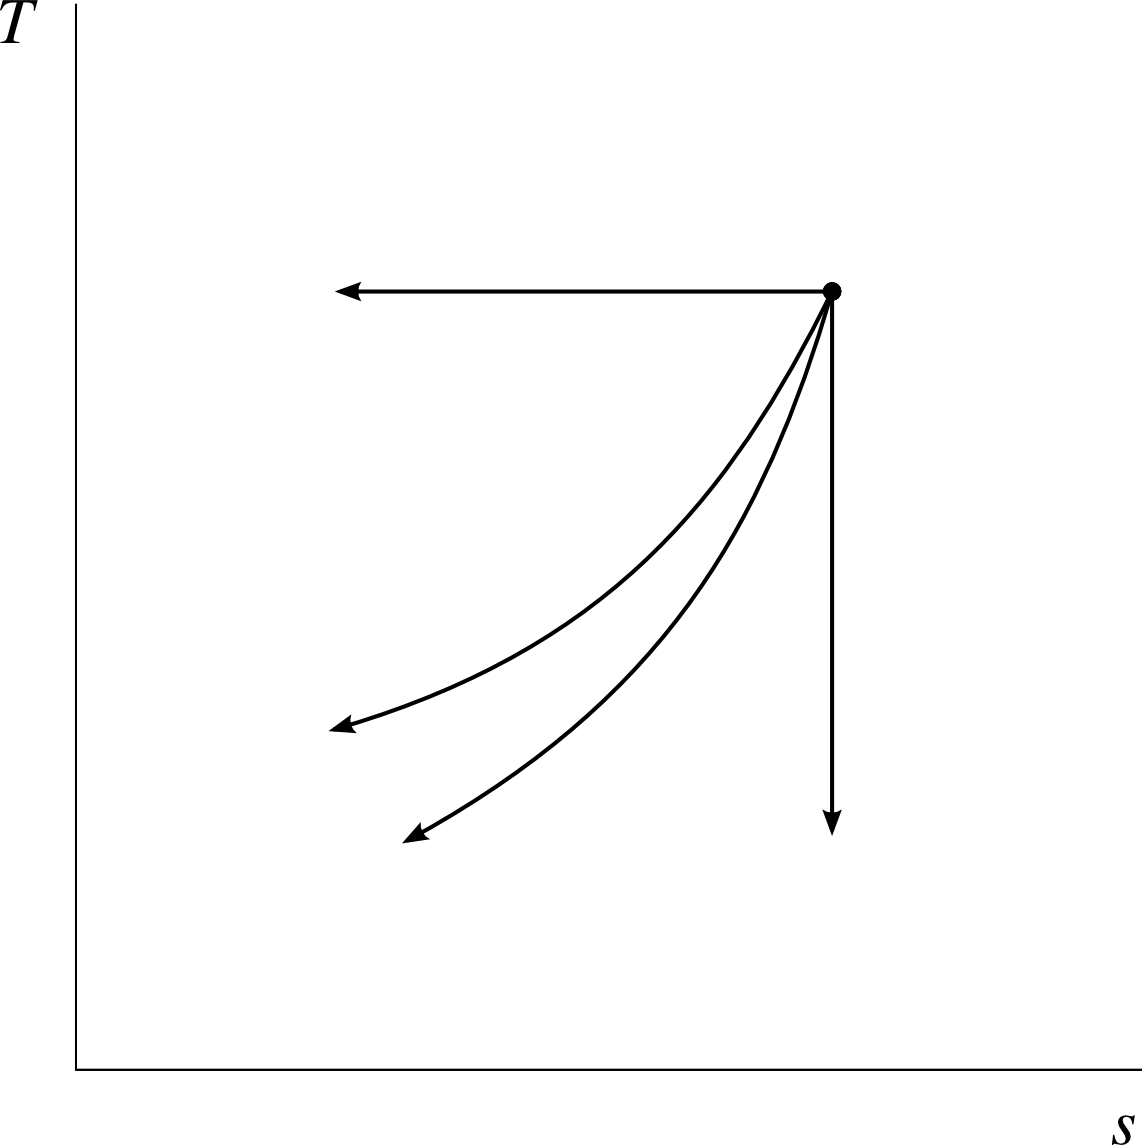
\includegraphics[width=0.6\columnwidth]{images/exo_ts_elementaires1.png}
			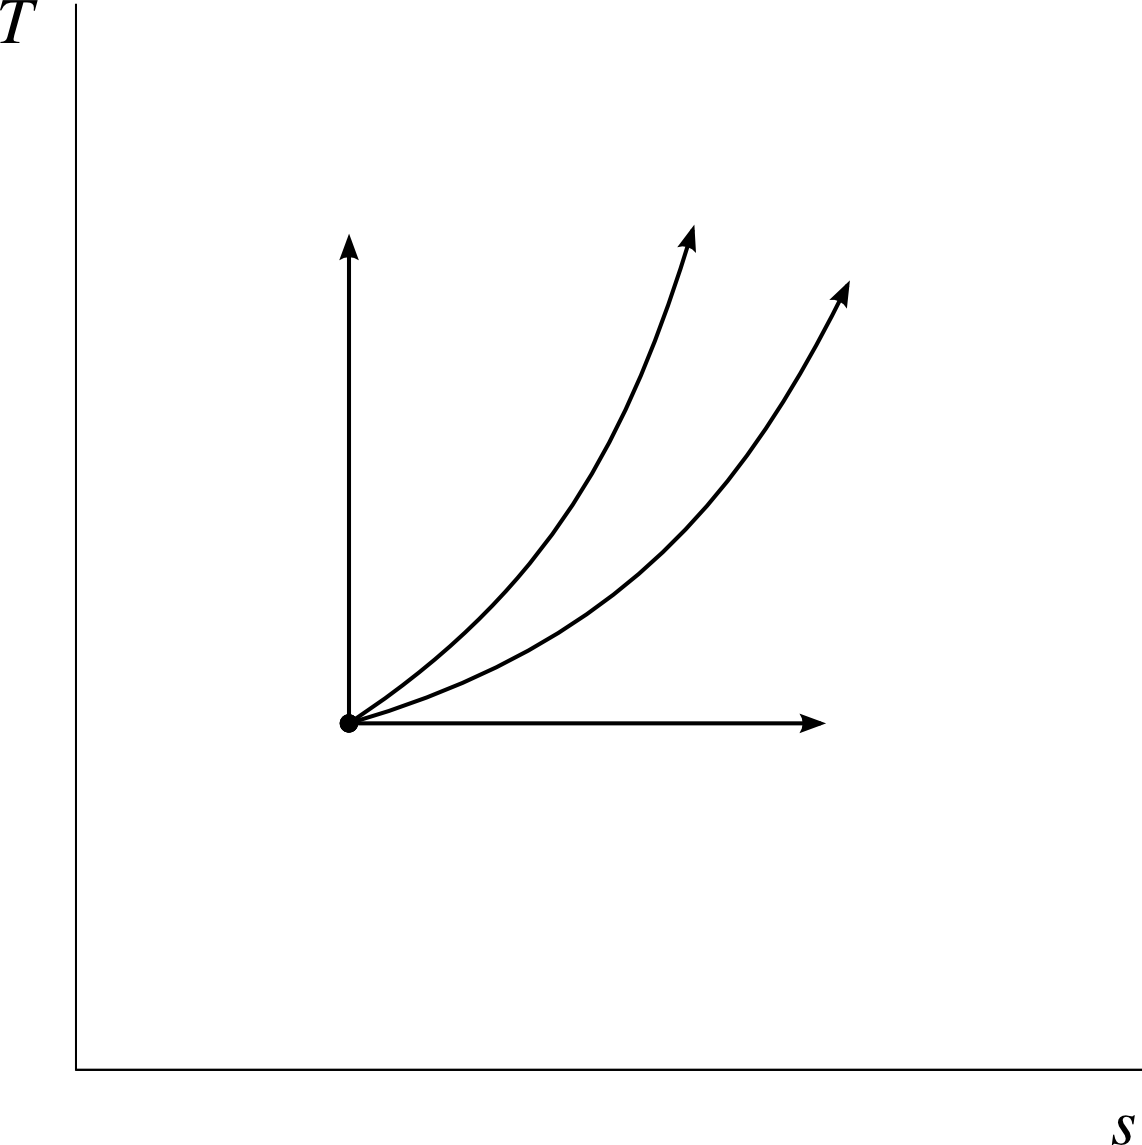
\includegraphics[width=0.6\columnwidth]{images/exo_ts_elementaires2.png}
		\end{center}
		\supercaption{Évolutions élémentaires réversibles d’un gaz parfait, représentées sur un diagramme température-entropie.}{schéma \cczero \oc}
		\label{fig_tsel}
	\end{figure}


\subsubsection{Détente d’un liquide/vapeur}
\label{exo_detente_liquide_vapeur}

	On dispose de~\SI{10}{\kilogram} d’eau à~\SI{45}{\bar} et~\SI{600}{\degreeCelsius}.
	
	\begin{enumerate}
		\item Quelle est la quantité maximale de travail qu’il est possible d’extraire de cette masse d’eau, sans lui fournir de chaleur, si on peut la détendre jusqu’à~\SI{4}{\bar} ?
		\item Si la détente était poursuivie jusqu’à une pression plus basse, à quelle température l’eau se condenserait-elle ?
		\item Représentez l’évolution sur un diagramme température-entropie, de façon qualitative (c’est-à-dire sans représenter les valeurs numériques), en y représentant aussi la courbe de saturation.
	\end{enumerate}


\subsubsection{Chauffage à température constante}
\label{exo_chauffage_isotherme_eau}

	On fournit lentement une quantité de chaleur de~\SI{3000}{\kilo\joule\per\kilogram} à une masse d’eau liquide saturée à~\SI{200}{\degreeCelsius}. La température est maintenue constante pendant toute l’évolution.
	
	Quelle est la quantité de travail développée par l’eau pendant l’évolution ? Représentez l’évolution sur un diagramme pression-volume, de façon qualitative en y représentant aussi la courbe de saturation.


\subsubsection{Diagrammes température-entropie}
\label{exo_diagrammes_ts}

	Représentez les évolutions que nous avons déjà étudiées, chacune sur un diagramme température-entropie, de façon qualitative en y faisant éventuellement figurer la courbe de saturation :
	
	\begin{enumerate}
		\item Évolutions simples : exercices \ref{exo_gp_isotherme} et \ref{exo_gp_isobare_isochore} p.\pageref{exo_gp_isobare_isochore}, \ref{exo_cours_vapeur_isotherme} et \ref{exo_generation_vapeur} p.\pageref{exo_generation_vapeur} ;
		\item Cycles thermodynamiques : exercices \ref{exo_moteur_carnot_vapeur} et \ref{exo_moteur_turbine_ideal} p.\pageref{exo_moteur_turbine_ideal}.
	\end{enumerate}

	
\subsubsection{Cycle de Carnot}
\label{exo_ts_carnot}

	Représentez le cycle suivi par le fluide à l’intérieur d’une pompe à chaleur opérant selon le cycle de Carnot sur un diagramme pression-volume, de façon qualitative et en y représentant aussi les deux transferts de chaleur.
	
	Comment le cycle serait-il modifié si la compression et la détente restaient adiabatiques mais n’étaient pas réversibles ? Comment seraient affectés les deux transferts de chaleur ?

\subsubsection{Turbine à vapeur}
\label{exo_turbine_vapeur_isentropique}

	Dans la salle des machines d’un navire important (\cref{fig_turbine_uss_hornet}), un débit de~\SI{250}{\tonne\per\hour} de vapeur rentre à~\SI{55}{\bar} et~\SI{660}{\degreeCelsius} dans la turbine.
	
	\begin{figure}[htp] %handmade
		\begin{center}
		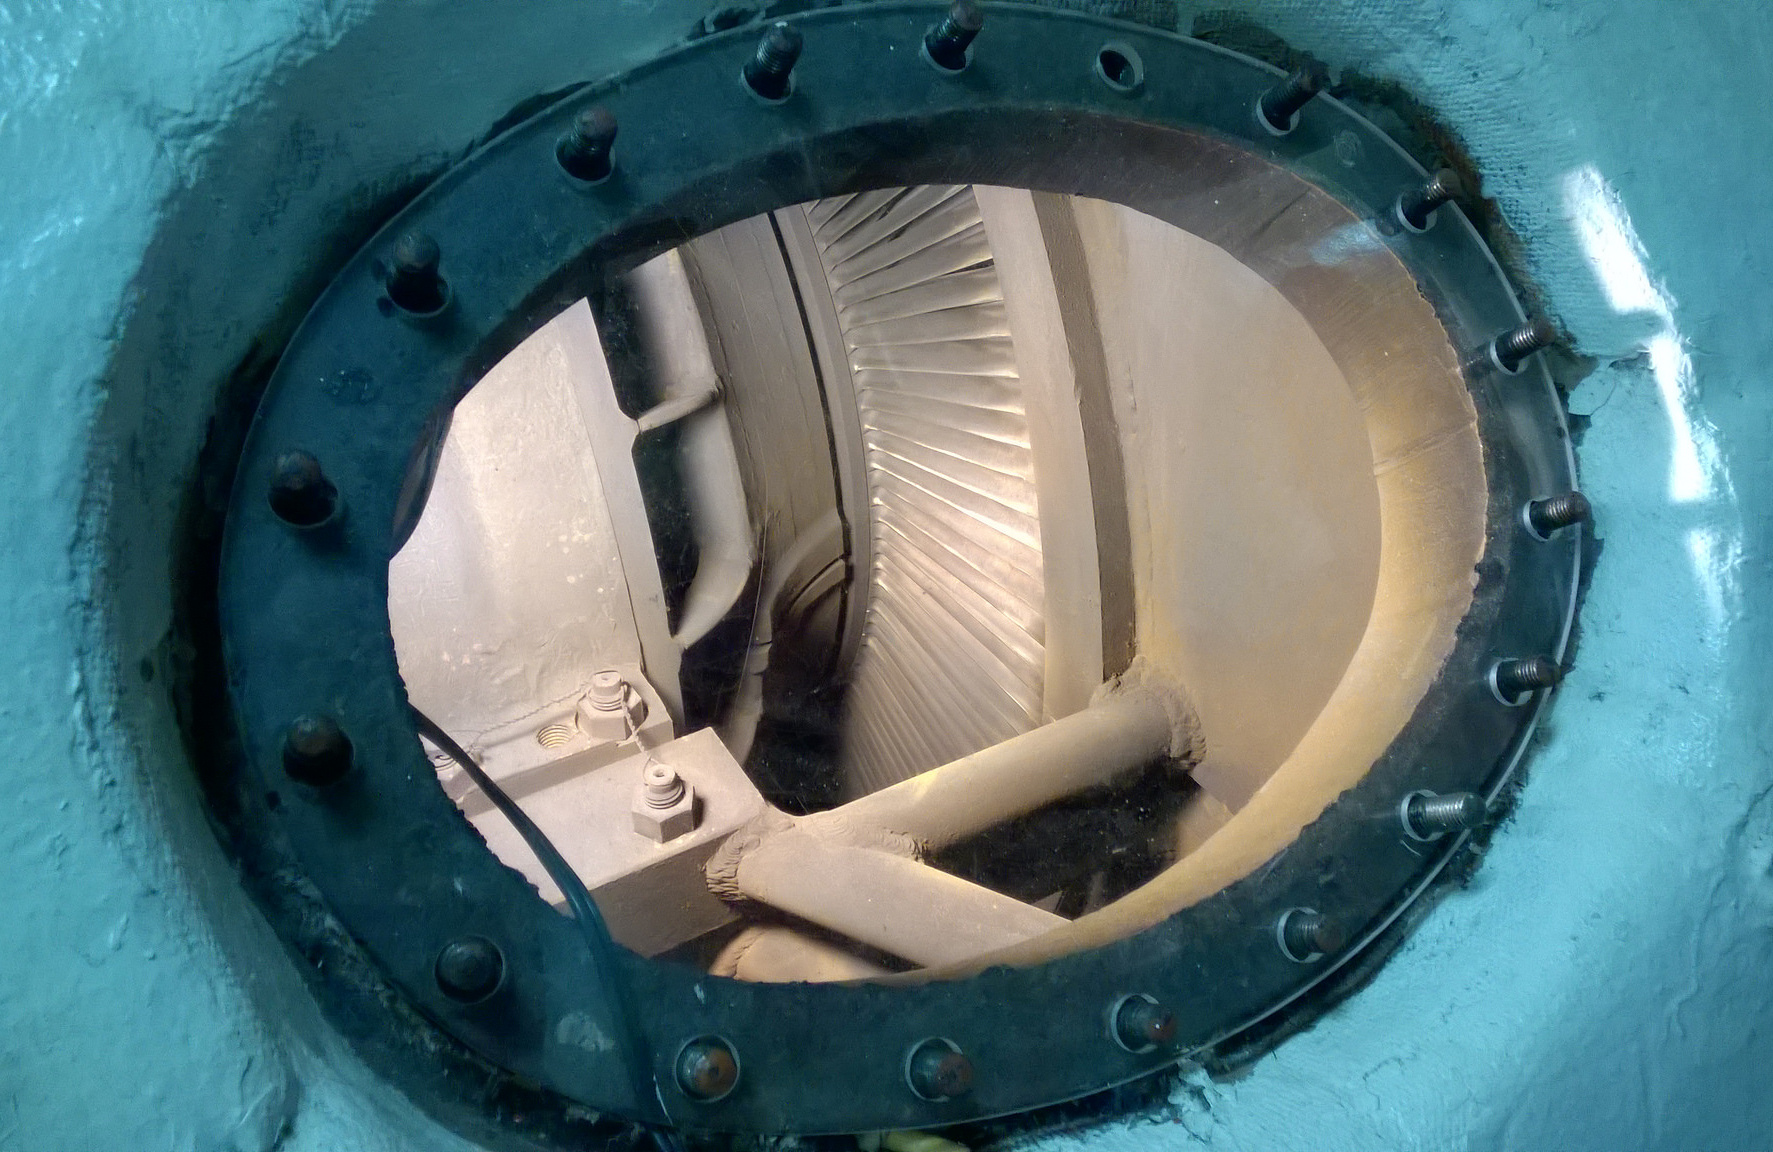
\includegraphics[width=\columnwidth]{images/turbine_uss_hornet.jpg}
		\end{center}
		\supercaption{Hublot d’inspection d’une des turbines basse pression (puissance \texttildelow\SI{25}{\mega\watt}) du porte-avions \textit{USS Hornet} lancé en 1943.}{\flickrfile{maralinga/15759249479}{Photo} \ccbysa par \flickrname{maralinga}{Tony Kent}}
		\label{fig_turbine_uss_hornet}
	\end{figure}
	
	Dans la turbine la vapeur est détendue en suivant une évolution approximativement adiabatique réversible. Lorsque la pression atteint \SI{1}{\bar}, on prélève de la vapeur avec un faible débit (\SI{1}{\kilogram\per\second}), pour réchauffer une autre partie de la centrale. La vapeur restant dans la turbine est détendue jusqu’à une pression de~\SI{0,18}{\bar}.
	
	Quelle est la puissance mécanique développée par la turbine ?

\subsubsection{Sens des transformations (1)}
\label{exo_sens_transfos_un}

	Une masse d’air suit une évolution sans apport de chaleur. Il y a deux états :
		\begin{itemize}
			\item Un état $X$ à~\SI{1}{\bar} et~\SI{300}{\degreeCelsius} ;
			\item Un état $Y$ à~\SI{5}{\bar} et~\SI{500}{\degreeCelsius}.
		\end{itemize}
		
	Quel est le seul sens ($X \to Y$ ou $Y \to X$) dans lequel l’évolution peut avoir lieu ?
	
	Représentez l’évolution sur un diagramme pression-volume et sur un diagramme température-entropie, de façon qualitative.

\subsubsection{Sens des transformations (2)}
\label{exo_sens_transfos_deux}

	De l’eau suit une évolution pendant laquelle on lui retire \SI{2}{\mega\joule\per\kilogram} de chaleur (sa température étant alors figée à~\SI{250}{\degreeCelsius}). Il y a deux états, un au début et l’autre à la~fin :
		\begin{itemize}
			\item Un état $X$ à l’état de vapeur saturée à~\SI{200}{\degreeCelsius} ;
			\item Un état $Y$ à l’état de liquide saturé à~\SI{240}{\degreeCelsius}.
		\end{itemize}
	Laquelle des deux évolutions doit avoir eu lieu avant l’autre ?

\subsubsection{Détente d’air comprimé}
\label{exo_detente_air_irreversible}

	L’air dans un cylindre isolé thermiquement est détendu depuis \SI{6,8}{\bar} et~\SI{430}{\degreeCelsius} jusqu’à~\SI{1}{\bar}.

	À la sortie, la température est mesurée à~\SI{150}{\degreeCelsius}.

	La détente est-elle réversible ? Représentez l’évolution sur un diagramme température-entropie, de façon qualitative.


\subsubsection{Pompe à air}
\label{exo_pompe_air}

	De l’air rentre dans une petite pompe centrifuge avec un débit de~\SI{4}{\kilogram\per\minute} (\cref{fig_pompe_stockholm}). La pompe n’est pas isentropique, mais on peut négliger ses pertes de chaleur.
	
	\begin{figure}[htp] %handmade
		\begin{center}
			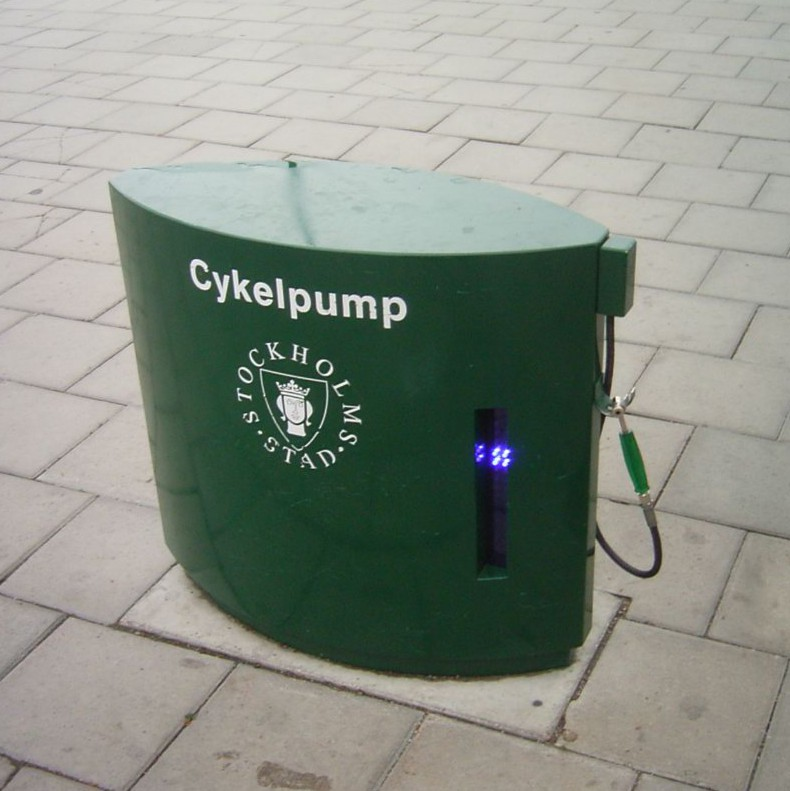
\includegraphics[width=0.6\columnwidth]{images/stockholm_pump.jpg}
		\end{center}
		\supercaption{Compresseur à air à usage public à Stockholm, destiné aux cyclistes. Un échangeur de chaleur intégré sous la carrosserie permet heureusement d’éviter les températures calculées dans cet exercice.}{Photo recadrée, \wcfile{Cykelpump-Stockholm.jpg}{version originale} \ccbysa \wdun{JakobVoss}{Jakob Voß}}
		\label{fig_pompe_stockholm}
	\end{figure}

	À l’entrée, l’air est à~\SI{1}{\bar} bar et~\SI{15}{\degreeCelsius}.\\
	À la sortie, la pression est à~\SI{2}{\bar} et on mesure la température à~\SI{97}{\degreeCelsius}.

	\begin{enumerate}
		\item Quelle est la puissance requise pour alimenter le compresseur ?
		\item Quelle serait la puissance si la compression se faisait de façon isentropique ?
		\item Quels seraient les transferts de chaleur et de travail nécessaires pour ramener l’air à ses conditions initiales (en minimisant les transferts de chaleur) ?
	\end{enumerate}

\subsubsection{Centrale électrique théorique}
\label{exo_cycle_carnot_vapeur}\index{Carnot!cycle de}\index{cycle!de Carnot}
	
	Pendant la conception d’une centrale électrique, un groupe d’ingénieurs enthousiastes étudie la possibilité de faire suivre à l’eau un cycle de Carnot. La chaleur dégagée par la combustion du charbon est transmise à une chaudière à vapeur. La vapeur est détendue dans une turbine, qui alimente une génératrice électrique.

	\begin{description}
		\item[De A à B] L’eau est compressée dans une pompe isentropique.\\
			En A, le mélange liquide-vapeur est à pression de~\SI{0,04}{\bar}.\\
			En B, l’eau est à l’état de liquide saturé, à pression de~\SI{40}{\bar}.
		\item[De B à C] L’eau est chauffée à pression constante (\SI{40}{\bar}) dans la chaudière.
			En C, l’eau est à l’état de vapeur saturée.
		\item[De C à D] L’eau est détendue dans la turbine isentropique.
			En D, l’eau est à la pression initiale, c’est-à-dire \SI{0,04}{\bar}.
		\item[De D à A] L’eau est refroidie dans un condenseur à pression constante (\SI{0,04} bar).
	\end{description}

\begin{enumerate}
	\item Schématisez les éléments du circuit suivi par la vapeur, et représentez l’évolution sur un diagramme température-entropie, de façon qualitative et en y représentant aussi la courbe de saturation.
	\item Quel est le titre de l’eau lorsque la condensation est interrompue (en A) ? Quelle est alors l’enthalpie spécifique ?
	\item Quel est le titre à la sortie de la turbine (en D) et l’enthalpie spécifique en ce point ?
	\item Quelle est la puissance développée par la turbine ?
	\item Quelle est la puissance de la chaudière ?
	\item Quelle est la puissance de la pompe ?
	\item Quel est le rendement de l’installation ?
\end{enumerate}


\subsubsection{Transferts de chaleur irréversibles}
\label{exo_transferts_chaleur_irreversibles}\index{température!gradient de}

	Un moteur à vapeur fonctionne sur un cycle de Carnot, avec un flux continu (débit :~\SI{2}{\kilogram\per\second}), entre les points de saturation de l’eau. Le moteur est conçu pour exploiter une source de chaleur de température modérée (\SI{300}{\degreeCelsius}), issue de la combustion de déchets industriels, et il rejette de la chaleur dans une rivière à basse température (\SI{5}{\degreeCelsius}).

	La chaudière a des parois épaisses pour réduire l’impact des imperfections de fabrication et pour soutenir la pression élevée de l’eau. Cette épaisseur impose un gradient de température important à travers les parois (\SI{10}{\degreeCelsius}). Il en va de même dans le condenseur (gradient :~\SI{10}{\degreeCelsius}).

	\begin{enumerate}
		\item De combien l’entropie de l’ensemble \{source de chaleur + eau\} augmente-t-elle ?
		\item De combien l’entropie de l’ensemble \{puits de chaleur + eau\} augmente-t-elle ?
		\item Quelle est la perte de puissance associée à cette augmentation d’entropie ?
		\item Quelle(s) propriété(s) du matériau constituant la chaudière sont-elles les plus désirables pour minimiser ce problème ?
	\end{enumerate}


\subsubsection{Compressions et détentes irréversibles}
\label{exo_compressions_detentes_irreversibles}

	L’équipe d’ingénieurs en charge du moteur de l’exercice précédent (cycle de Carnot fonctionnant entre \SI{290}{\degreeCelsius} et~\SI{15}{\degreeCelsius}, exercice~\ref{exo_transferts_chaleur_irreversibles}) découvre que les phases de compression et détente ne se font pas de façon réversible.

	Le compresseur amène bien l’eau à température haute mais sa consommation de travail est \SI{10}{\percent} plus importante que prévu. La turbine amène bien l’eau à température basse, mais elle fournit \SI{10}{\percent} d’énergie mécanique en moins que prévu.
	
	\begin{enumerate}
		\item De combien l’entropie de la vapeur augmente-t-elle dans chacun de ces deux composants ?
		\item De combien augmentent les rejets de chaleur ?
		\item Quelle est la perte en efficacité de l’installation par rapport à une installation réversible ?
	\end{enumerate}


\exercisesolutionpage
\titreresultats

	\begin{description}
		\item [\ref{exo_questions_cours}]
						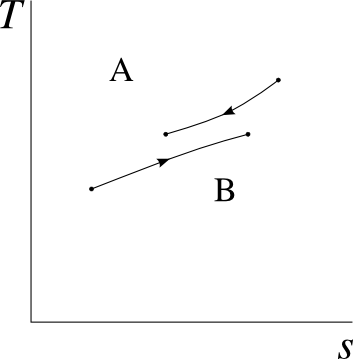
\includegraphics[width=\solutiondiagramwidth]{images/exo_sol_ts_tasse.png}
						\tab 1) Voir \S\ref{ch_entropie_definition} p.\pageref{ch_entropie_definition} ;
						\tab 2) Oui bien sûr, un simple prélèvement de chaleur suffit : voir à ce propos l’exemple~\ref{exemple_delta_entropie_basics} p.\pageref{exemple_delta_entropie_basics} ;
						\tab 3) Capacité thermique massique : chaleur spécifique $\diff q$ nécessaire pour générer une variation $\diff T$ de température (\cref{eq_def_capacité_calorifique_massique} p.\pageref{eq_def_capacité_calorifique_massique} : $c\ \equiv \ \frac{\diff q}{\diff T}$). Entropie massique : chaleur spécifique $\diff q$ \emph{divisée par la température} à laquelle elle est fournie, pendant une évolution réversible (\cref{eq_variation_franche_entropie} p.\pageref{eq_variation_franche_entropie}) ;
						\tab 4) Les deux températures évoluent jusqu’à s’égaliser ; $\Delta s_\A + \Delta s_\B > 0$.
		\item [\ref{exo_ts_variations_elementaires}]
						\tab \textit{Dans le sens horaire, en partant de la verticale, sur les deux graphiques :} isentropique, isochore, isobare, isotherme.
		\item [\ref{exo_detente_liquide_vapeur}]
						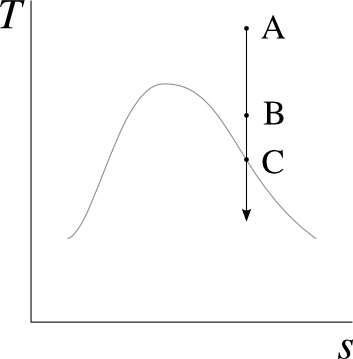
\includegraphics[width=\solutiondiagramwidth]{images/exo_sol_ts_detente_eau.png}
						\tab\tab 1) $u_1 = \SI{3276,4}{\kilo\joule\per\kilogram} $ et $u_2 = \SI{2703,3}{\kilo\joule\per\kilogram}$ : $W_\text{max.} = \SI{-5,731}{\mega\joule}$.
						\tab 2) $T_3 = \SI{103,51}{\degreeCelsius}$
		\item [\ref{exo_chauffage_isotherme_eau}]
						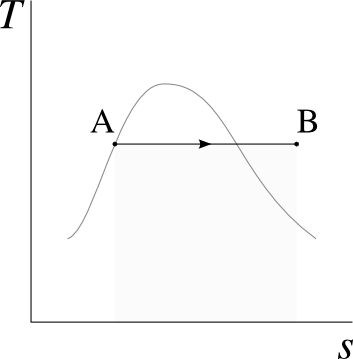
\includegraphics[width=\solutiondiagramwidth]{images/exo_sol_ts_chauffage_isotherme_eau.png}
						\tab\tab $s_2 = \SI{8,671}{\kilo\joule\per\kelvin\per\kilogram}$ ; ainsi $u_2 = \SI{2660,89}{\kilo\joule\per\kilogram}$ ; enfin $w_{1\to 2} = \SI{-1,19}{\mega\joule\per\kilogram}$.
		\item [\ref{exo_diagrammes_ts}]
						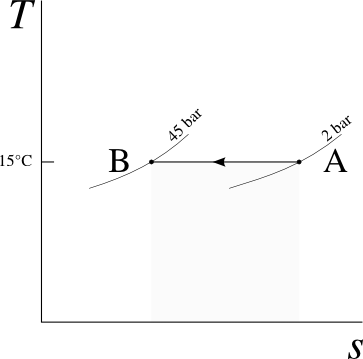
\includegraphics[width=\solutiondiagramwidth]{images/exo_sol_ts_multiples1.png}
						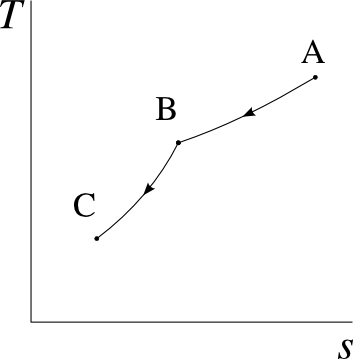
\includegraphics[width=\solutiondiagramwidth]{images/exo_sol_ts_multiples2.png}
						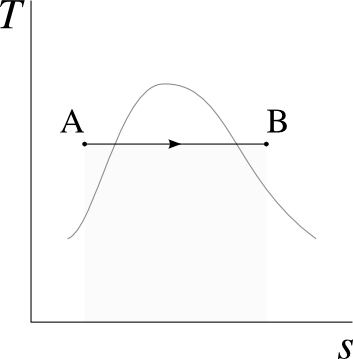
\includegraphics[width=\solutiondiagramwidth]{images/exo_sol_ts_multiples3.png}
						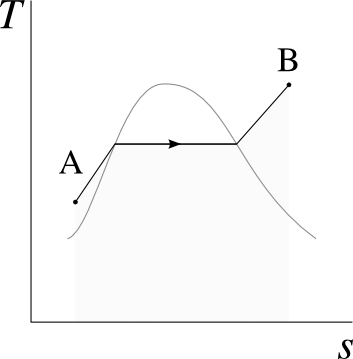
\includegraphics[width=\solutiondiagramwidth]{images/exo_sol_ts_multiples4.png}
						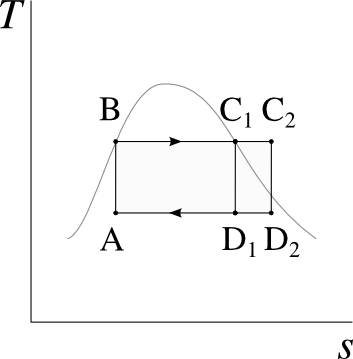
\includegraphics[width=\solutiondiagramwidth]{images/exo_sol_ts_multiples5.png}
						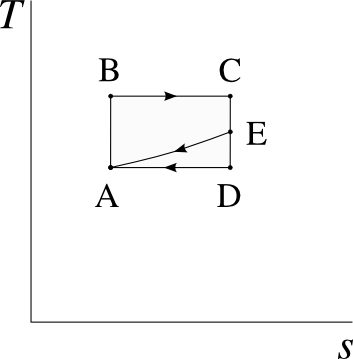
\includegraphics[width=\solutiondiagramwidth]{images/exo_sol_ts_multiples6.png}
		\item [\ref{exo_ts_carnot}]
						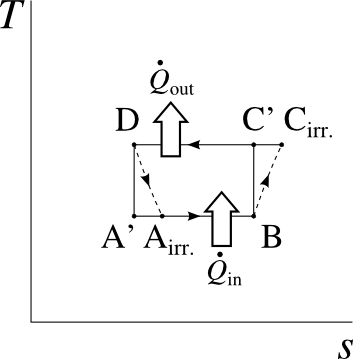
\includegraphics[width=\solutiondiagramwidth]{images/exo_sol_ts_carnot_thermopompe.png}
						\tab 2) Dans ce cas $W_{\B\to\C_\text{irr.}} > W_{\frombtoc’}$ et, en valeurs négatives, $W_{\D\to\A_\text{irr.}} > W_{\fromdtoa’}$. Ainsi la chaleur à rejeter $Q_{\fromctod}$ augmente (ce qui peut au premier abord sembler un résultat intéressant) et la chaleur prélevée $Q_{\fromatob}$ diminue (et l’on voit que l’augmentation de $Q_{\fromctod}$ ne provient en fait que des inefficacités du compresseur et de la turbine, et ne fait que diminuer le rendement).
		\item [\ref{exo_turbine_vapeur_isentropique}]
						\tab La démarche est comme décrite dans l’exemple~\ref{exemple_turbine_vapeur_isentropique} p.\pageref{exemple_turbine_vapeur_isentropique} : $h_1 = \SI{3803,5}{\kilo\joule\per\kilogram}$ (vapeur sèche) ; $h_2 = \SI{2677,7}{\kilo\joule\per\kilogram}$ (vapeur sèche) ; $h_3 = \SI{2413,6}{\kilo\joule\per\kilogram}$ (mélange de titre \SI{91,9}{\percent}) ; on a donc $\dot{W}_\text{turbine} = \SI{-96,26}{\mega\watt}$.
		\item [\ref{exo_sens_transfos_un}]
						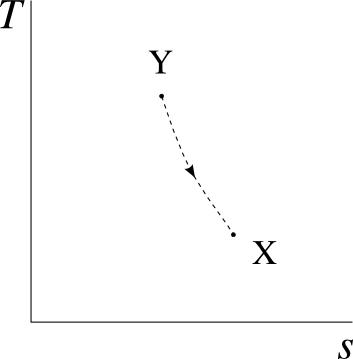
\includegraphics[width=\solutiondiagramwidth]{images/exo_sol_ts_bonsens1.png}
						\tab\tab Avec l’\cref{eq_delta_s_gp_p} on constate que $s_Y - s_X = \SI{-161,08}{\joule\per\kelvin\per\kilogram} < \int_X^Y \left(\frac{\diff q}{T}\right)_\text{chemin réel} = \SI{0}{\kilo\joule\per\kelvin\per\kilogram}$ (puisque l’évolution est adiabatique). Ainsi le sens est $Y\to X$.
		\item [\ref{exo_sens_transfos_deux}]
						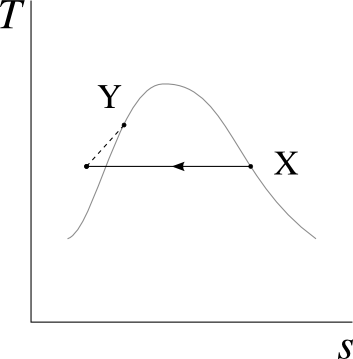
\includegraphics[width=\solutiondiagramwidth]{images/exo_sol_ts_bonsens2.png}
						\tab On suppose $X\to Y$, alors $\Delta s = \SI{-3,728}{\kilo\joule\per\kelvin\per\kilogram}$ mais $\int_X^Y \left(\frac{\diff q}{T}\right)_\text{chemin réel} = \SI{-3,823}{\kilo\joule\per\kelvin\per\kilogram}$ ainsi nous sommes rassurés : le sens est bien $X\to Y$.
		\item [\ref{exo_detente_air_irreversible}]
						\tab Avec l’\cref{eq_delta_s_gp_p}, nous obtenons $\Delta s = \SI{+39,77}{\joule\per\kelvin\per\kilogram}$ mais --\textit{aha}!-- $\int_1^2 \left(\frac{\diff q}{T}\right)_\text{chemin réel} = \SI{0}{\kilo\joule\per\kelvin\per\kilogram}$, ainsi la transformation est irréversible. Nous aurions également pu utiliser la fort classique équation~\ref{eq_isentropique_horrible2} p.\pageref{eq_isentropique_horrible2} pour découvrir que $T_{2 \text{isentropique}} < \SI{150}{\degreeCelsius}$.
		\item [\ref{exo_pompe_air}] 	
						\tab 1) $\dot{W}_\text{pompe} = \dot m c_p \Delta T = \SI{+5,493}{\kilo\watt}$ (\ref{eq_petite_sfee_deltas_h} \& \ref{eq_h_fonction_de_T}) ;
						\tab 2) Avec l’équation~\ref{eq_isentropique_horrible2} $T_{2 \text{is.}} = \SI{351,3}{\kelvin}$ soit tout de même \SI{78,1}{\degreeCelsius}, ainsi $\dot{W}_\text{idéal} = \SI{+4,231}{\kilo\watt}$ ;
						\tab 3) Une possibilité : détente isentropique pour obtenir $\dot{W}_{2\to 1} = \SI{-4,231}{\kilo\watt}$, puis un nécessaire refroidissement sans travail de $\dot{Q}_{2\to 1} = \SI{-1,262}{\kilo\watt}$. Toutes les transformations réversibles dont la somme nette des transferts prend ces valeurs (par exemple lors d’une détente refroidie) permettront de revenir en 1.
		\item [\ref{exo_cycle_carnot_vapeur}]
						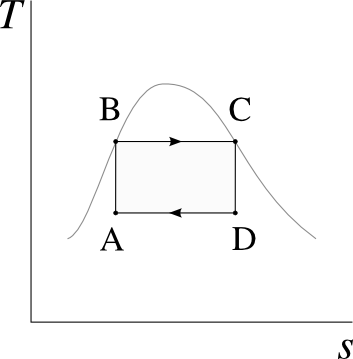
\includegraphics[width=\solutiondiagramwidth]{images/exo_sol_ts_carnot_vapeur1.png}
						\tab L’agencement est représenté en~\cref{fig_exo_carnot_circuit_vapeur} p.\pageref{fig_exo_carnot_circuit_vapeur} ;
						\tab\tab 2) $x_\A = \frac{s_\B - s_L}{s_{LV}} = \num{0,2949}$ ; ainsi $h_\A = h_L + x_\A h_{LV} = \SI{838,7}{\kilo\joule\per\kilogram}$ ;
						\tab 3) Même démarche : $x_\D = \num{0,7014}$ ainsi $h_\D = \SI{1827,5}{\kilo\joule\per\kilogram}$ ;
						\tab 4) $w_\text{turbine} = h_\D - h_\C = \SI{-973,3}{\kilo\joule\per\kilogram}$ ;
						\tab 5) $q_\text{chaudière} = h_\C - h_\B = \SI{+1713}{\kilo\joule\per\kilogram}$ ;
						\tab 6) $w_\text{pompe} = h_\B - h_\A =  = \SI{+248,8}{\kilo\joule\per\kilogram}$ ;
						\tab 7) $\eta_\text{centrale} = \left|\frac{w_\net}{q_\inn}\right| = \frac{-w_\text{turbine} - w_\text{pompe}}{q_\text{chaudière}} = \SI{42,29}{\percent}$. Comme toutes les phases sont réversibles et que les transferts de chaleur sont isothermes, on a bien $\eta_\text{centrale} = \eta_\text{moteur carnot} = 1 - \frac{T_\text{eau condenseur}}{T_\text{eau chaudière}}$ (\ref{eq_efficacité_moteur_carnot_température}).
		\item [\ref{exo_transferts_chaleur_irreversibles}]
						\tab 1) $\dot{S}_\text{paroi haute température} = \dot{m} \ (\Delta s_\text{combustion} + \Delta s_\text{eau}) = \SI[per-mode = symbol]{+91,77}{\joule\per\kelvin\per\second} = \SI{+91,77}{\watt\per\kelvin}$ ;
						\tab 2) $\dot{S}_\text{paroi basse\ température} = \SI{+188,3}{\watt\per\kelvin}$, et l’on voit qu’un gradient de~\SI{10}{\degreeCelsius} est plus pénalisant à basse température qu’à haute température ;
						\tab 3) $\dot{W}_\text{perdue} = \dot Q_\inn \left(\eta_\text{supérieure} - \eta_\text{inférieure}\right) = \SI{77,9}{\kilo\watt}$
						\tab 4) Pour réduire les gradients de température, il faut des matériaux avec une très grande conduction thermique (ce n’est bien sûr pas la seule qualité qui leur est demandée…).
		\item [\ref{exo_compressions_detentes_irreversibles}]
						\tab 1) $\Delta s_\text{compresseur} = \SI{+67}{\joule\per\kelvin\per\kilogram}$ ; $\Delta s_\text{turbine} = \SI{+382}{\joule\per\kelvin\per\kilogram}$ ;
						\tab 2) $\Delta q_\out = \SI{-110,2}{\kilo\joule\per\kilogram}$ soit \SI{+14,6}{\percent} ;
						\tab 3) $\eta_\text{installation réelle} =\SI{39,82}{\percent}$, soit \SI{-9}{pt}.
	\end{description}
